\chapter{Решение поставленной задачи}

\section{Анализ текста решения}

\subsection{ANTLR}
Для синтаксического анализа решения предлагается использовать генератор анализаторов для формальных языков ANTLR.
Чтобы получить парсер нужного языка, достаточно просто передать грамматику для данного языка в нужном формате.
ANTLR зарекомендовал себя как стабильное и удобное средство для работы с синтаксическим анализом, при этом
обладая крайне полезными для представленной работы приемуществами:
\begin{itemize}
    \item Свободное программное обеспечение.
    \item Использование единой нотации для описания лексических и синтаксических анализаторов.
    \item В репозитории разработчиков есть примеры грамматик для многих популярных языков программирования.
    \item Множество плагинов для работы в различных средах разработки, в том числе и для Intellij IDEA, которая
        использовалась в данной работе.
    \item Возможность добавлять Java-код в грамматику с целью подстановки его напрямую в парсер. При помощи этого 
        можно запрограммировать парсер возвращать какую-угодно информацию о тексте.
    \item Предоставление сообщений об ошибках и восстановление после них, в том числе корректная обработка отсутствующих узлов, 
        с последующим продолжением работы над остальным текстом. 
\end{itemize} 

Основной сложностью при работе с ANTLR стало то, что он не умеет по дереву разбора восстанавливать исходный код программы, так
как все пробелы и разделители убираются при работе лексера, и никаких обратных приобразователей не генерируется. Также проблемой
стало отсутствие возможности как-либо модифицировать построенные деревья разбора, однако обе эти проблемы решаемы.

Чтобы решить возникшие проблемы, можно модифицировать стандартную реализованную грамматику из репозитория разработчиков
добавив код, который будет строить дерево разбора, методы и структуру для которого можно реализовать отдельно на языке
Java.

После модификации грамматики работа с ANTLR сводится к нажатию пары кнопок для генерации лексера и парсера. 

\subsection{Выбор языка программирования}

Так как работать планируется со структурой кода при помощи деревьев разбора, можно не умаляя общности рассматривать один
конкретный язык программирования. Для добавления другого языка нужно будет лишь использовав новую грамматику получить новые лексер
и парсер, а также запрограммировать элементы структуры дерева разбора.

В данной работе будет рассматриваться язык программирования Паскаль. Это один из наиболее популярных языков для олимпиад
по программированию, который долгое время использовался для начального обучения школьников и студентов. В момент написания
работы, язык программирования сдал лидирующие позиции, однако все еще популярен и используется даже на всероссийской олимпиаде
школьников по программированию (РОИ). Язык дорабатывается по сей день в рамках языков Pascal ABC и Delphi.

Паскаль имеет следующие оссобенности:
\begin{itemize}
    \item Строгая типизация.
    \item Структурное программирование.
    \item Текстовая простота.
\end{itemize}

При программировании на Паскале может сложиться ощущение, что вы программируете на английском языке, настолько синтаксис оптимизирован
для обучения.

В представленной работе будет рассмотрено избыточное подмножество изначального стандарта языка 
<<Pascal Standard>>, принятого в 1974 году.

\begin{algorithm}[!h] 
\caption{Пример программы на языке Паскаль}\label{lst1} 
\begin{lstlisting}[language=pascal]
program tmp;
const
  Author = 'Grigory';
var
  arr: array[1..2] of string;
begin
  writeln('Hi')
end.
\end{lstlisting} 
\end{algorithm}

\subsection{Дерево разбора}

Для работы с деревьями разбора по причинам, описанным ранее, необходимо было разработать собственную структуру данных, представляющую
дерево разбора, при этом позволяющую изменять свою структуру и получать код программы, которой это дерево отвечает.

Разработка данной структуры проводилась на языке программирования Java. Этот язык объектно ориентированный, что положительно сказалось
на дизайне кода и удобстве его написания, а также ANTLR, как уже отмечалось, отлично с ним совместим.

Структура данных наследуется из основного общего класса \texttt{ASTNode}, который представляет из себя вершину дерева.
Основные типы вершин это:
\begin{itemize}
    \item переменная;
    \item константа;
    \item функция;
    \item процедура;
    \item условие;
    \item цикл с предусловием;
    \item цикл с постусловием; 
    \item цикл со счетчиком;
    \item перечисление (код между \texttt{begin} и \texttt{end});
    \item текст;
    \item тип.
\end{itemize}
Также есть вспомогательные:
\begin{itemize}
    \item двоичная операция;
    \item унарная операция;
    \item скобки;
    \item строка;
    \item универсальная.
\end{itemize}

Универсальная вершина разработана для удобства, через вершину данного типа можно разработать любую вершину, у которой есть дети.
От нее наследуются, например, вершины двоичной и унарной операций, а также вершиана перечислений.  

Данная структура предназначена для представления конкретно выбранного языка, но несложно дополняется для поддержки дополнительной
функциональности языка, либо другого языка.

\begin{figure}[!h] 
\caption{Пример дерева разбора для программы из листинга~\ref{lst1}}\label{fig1} 
\begin{center}
  \makebox[\textwidth]{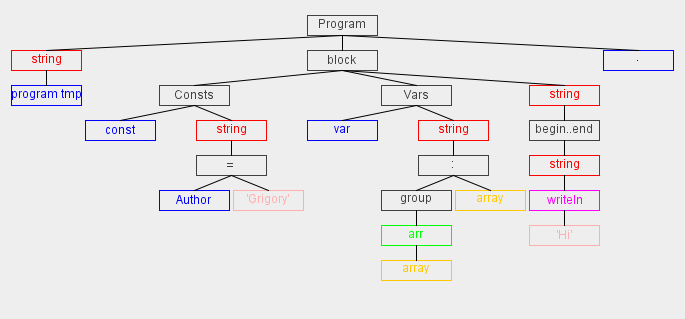
\includegraphics[width=0.9\paperwidth]{pics/tree-example.png}}
\end{center}
\end{figure}

Как было отмечено ранее, ANTLR поддерживает вставки Java-кода, поэтому стандартная грамматика была модифицирована для поддержки
разработанной структуры данных. Пример приведен в листинге~\ref{lst2}. 

\begin{algorithm}[!h] 
\caption{Пример грамматики ANTLR с вставками Java-кода}\label{lst2} 
\begin{lstlisting}[basicstyle=\small] 
constant returns [ASTNode ast]
 :unsignedNumber {
   $ast = new ConstNode($unsignedNumber.text, "num");
  }
 |sign unsignedNumber {
   $ast = new ConstNode($sign.text + $unsignedNumber.text, "sNum");
  }
 |identifier {
   $ast = new ConstNode($identifier.text, "id");
  }
 |sign identifier {
   $ast = new ConstNode($sign.text + $identifier.text, "sId");
  }
 |string {
   $ast = new ConstNode($string.text, "str");
  }
 ; 
\end{lstlisting} 
\end{algorithm}

В представленной структуре для каждого поддерева реализован метод \texttt{toString}, который сопоставляет ему
корректный код программы, который репрезентует данное поддерево. 

\section{Работа с деревьями разбора}

\subsection{Поиск исправления}

Имеется два решения участника. Построим для них деревья разбора, представленные структурой данных, описанной выше, 
с помощью имеющегося парсера. Также вспомним, что 

\chapterconclusion

\begin{enumerate}
    \item ...
\end{enumerate}
